%\chapter*{Cryptography}


Cryptography(classical greek for \textit{krypt\^{o}s}, which means \textit{concealed})
is the science of encrypting information.
Related to computer engineering, it is the art of hiding information by turning cleartext
data into a 
pseudo-random looking stream or block of bits, called ciphertext, using some kind of
\textit{key}. This process is called \textit{encryption}.
Unauthorized parties - lacking the used key - should, by looking at the ciphertext, learn
absolutely nothing about the hidden cleartext. Authorized parties, on the other hand, are
able to retrieve the original data out of the ciphertext by using the key, and thus reversing
the encryption. This reversing process is called \textit{decryption}.
\\

This way, cryptography is used to provide these objectives:

\begin{itemize}
 \item Privacy / Confidentiality: protected data can only be read by authorized parties
 \item Integrity: ensuring that information has not been altered, or altering can be detected
 \item Authenticity: the origin of the data is genuine
 \item Non-Repudiation: prevent an entity from denying commitments or actions how had been 
 granted earlier
\end{itemize}

FIXME: comutationally secure vs. unconditionally secure, i.e. one time pad(perfect secrecy?)
FIXME: MERKLE puzzles

A fundamental goal of cryptography is to provide all of these 4 objectives. Providing these
objectives only partially will not result in a secure system. For example, providing privacy and
integrity, but no authenticity, may lead to so called 'replay' attacks, as will be shown.
FIXME: replay attack

To be able to make rigorous statements, it is important to introduce some basic background knowledge, which
is given in the next chapter:

\subsection{Propabilistic Theory}

\section{History of Cryptography}
FIXME:BIBLOGRAPHY: the codebreakers

The evolution of cryptography was no linear process. Ciphers were used independently in different
places, were forgotten and disappeared when the corresponding civilization died. Nevertheless,
basics are found thousands of years ago, therefore a short time line showing some noteable
events is presented below:

\begin{itemize}
 \item Egypt, about 2000 B.C.: a simple substitution is used to partially replace ordinary hieroglyphs with special ones. 
 \item Sparta, about 500 B.C.: a device called 'skytale' is used to encrypt military messages
 \item Rome, about 100 B.C.: Caesar uses a simple substitution cipher for military correspondence, replacing every
 letter of the alphabet with the letter 4 places further down the alphabet
 \item China, 11th century: for a list of 40 items, the first 40 ideograms of a poem are assigned
 \item Arabia, 14th century: 7 different ciphers and the frequency analysis of letters are
 introduced by Ahmas al-Qalqashandi
 \item Vienna, 17th century: the 'Geheime Kabinets-Kanzlei' routinely intercepts, copies and 
 re-seales diplomatic correspondence to embassies, and manages to decrypt a great percentage of the ciphertexts   
 \item England, 19th century: Samuel F.B. Morse invents the Morse Code
 \item England, 1940: the so called 'Turing Bomb', an electromechanical device, is used to decrypt
 German Enigma-based ciphertexts
 \item USA, 1976: Whitfield Diffie and Martin Hellman specify the a protocol for key exchange,
 based on a public key system developed by Ralph Merkle
 \item USA, 1977: RSA public key encryption is defined
 \end{itemize}

 
\section{Definitions and Basic Assumptions}

\begin{itemize}
 \item $\mathcal{A}$ is a finite set, denoting the alphabet used, for example
 $\mathcal{A} = \{0, 1\}$
 \item $\{0, 1\}^n$ denotes the set of all possible strings with length $n$
 \item $\mathcal{M}$ is the message space, consisting of all strings that can be built with the 
 underlying alphabet
 \item $\mathcal{C}$ is the ciphertext space, also consisting of the strings from 
 the alphbet
 \item $\mathcal{K}$ is called keyspace, also built from the alphabet. Every element
 $e \in \mathcal{K}$ is called a key and determines the function $\mathcal{M} \rightarrow \mathcal{C}$.
 This function, $E_e$ is called the \textit{encryption function}. 
  \begin{center}
 $ciphertext = E_e(e, cleartext)$
  \end{center}

 \item For every key $d \in \mathcal{K}$, $D_d$ denotes the function from $\mathcal{C} \rightarrow
  \mathcal{M}$, and is called \textit{decryption function}.
  \begin{center}
  $cleartext  = D_d(d, ciphertext)$
    \end{center}
 \item The keys $e$ and $d$ are also referred to as \textit{keypair}, written $(e,d)$. 
 
 \item If it is computationally easy to derive the private key $e$ from the public key $d$(in most cases $e = d$), the encryption scheme
 is called \textit{symmetric}, otherwise the scheme is called \textit{asymmetric}.
 \item A cipher(also called \textit{encryption scheme}) defined over $\mathcal{(K,M,C)}$ is a pair of \textit{efficient}
 \footnote{'runs in polynomial time   FIXME: erklären?} algorithms s.t.
 \begin{center}
   $\mathcal{K} \times \mathcal{M} \rightarrow \mathcal{C}$
   \\
   $\mathcal{K} \times \mathcal{C} \rightarrow \mathcal{M}$
 
 \end{center}

 \item Correctness property / Consistency equation: for every pair of $(e,d) \in \mathcal{K}$ and for every message $m \in \mathcal{M}$ it must hold that 
 \begin{center}  
 $ m = D_d(d, (E_e(e, m))$
  \end{center}
  
 \item An \textit{advisory} is a entity, not owning the keypair, which is trying to break a cipher, i.e. systematically trying to decode ciphertexts.  
 \item A \textit{secure} cipher is a cipher for which it is provable that no attack in whatsoever form exists on this cipher 
\end{itemize}

According to \textit{Kerckhoff's Principle}, stated by the dutch cryptographer Auguste Kerckhoff in 1883, a secure system should not rely on the secrecy of
its components, the only part that should be kept secret is the key alone. Mapped to the definitions above, the sets $\mathcal{M, C, K}$, as well as the
transformation functions $E_e$ and $D_d$, must not secret. The only thing that has to be kept private is the keypair $(e, d)$.

FIXME: vergleich security by obscurity

\section{Kind of Ciphers}

Two main kinds of ciphers exist, stream- and blockciphers:

\subsection{Stream Ciphers}

For encryption, stream ciphers take arbitrary long messages(from the message space $\mathcal{M}$), and encrypt
them to the corresponding ciphertext(out of the ciphertext-space $\mathcal{C}$), by applying
one digit of the message to one digit of the key. It is valid to say that a streamcipher is a block cipher with blocklength 1.

\begin{itemize}
 \item A keystream is a sequence of symbols $e_0, e_1, ..., e_n$, all taken from the keyspace $\mathcal{K}$
\end{itemize}

The encryption function $E_e$ performs the substitution $c_i = E_e(e_i, m_i)$, producing one encrypted symbol at a time. Analogously,
the decryption function inverts this substitution: $m_i = D_d(d_i, c_i)$, with $e_i = d_i$, which means that this kind of cipher is a
symmetric one.

\subsubsection{Secure Ciphers - The one time pad}

As a first example of a theoretically secure cipher the so called 'one time pad' is introduced. This cipher was invented
by Gilbert Vernam in 1970, and belongs to the family of stream ciphers. 


\subsection{Shannons Communication Theory}

FALSCH: keylength >= message -> secure
It is important to state that attacks on any cipher are always possible: the so called
'Exhaustive Attack' will always find the proper key in the long run, just by trying every
possible key - no matter what kind of encryption is used. So, this most naive attack will always work, but
will not finish in feasible time if a proper key(or more concrete: a proper key-length) is used, turning this bruteforce-attack
impracticable. Nevertheless, this statement says that it is principly impossible to design
a cipher which can \textit{never} get broken.

\subsection{Block Ciphers}

Here, the cleartext-message is broken into equally sized parts, which are then encrypted block by block. While streamciphers are not parallelizable
by nature, there exist methods to speed up en- and decryption by splitting the message respectively ciphertext first as normal, and then process them in
parallel\footnote{Counter Mode, see \ref{confidentiality}}. A disadvantage of block ciphers is that it may be necessary to pad the last block to the used block size. 
\\
\\
Three main groups of block cipher exists:
\begin{itemize}
 \item Permutation Blockciphers
 \item Substitution Blockciphers
 \item Product Blockciphers
 \item Feistel Networks
\end{itemize}

\subsubsection{Permutation Blockciphers}

\subsubsection{Substitution Blockciphers}

\subsubsection{Product Blockciphers}

\subsection{Feistel Networks}

\subsection{Stream Ciphers}

\subsection{Block Ciphers}

\subsection{Confidentiality}\label{confidentiality}

\subsubsection{Cipher Block Chaining - CBC}

For encryption, CBC needs as underlying block cipher which is invertible, so a PRP has to be used. 
As usal, the message has to be broken into blocks, suitable for the block cipher. 

\begin{center}
$ C_0 = E(k, (M_0 \bigoplus IV ) )  $
\\
$ C_1 = E(k, (M_1  \bigoplus C_0) ) $
\\
$...$
\\
$ C_i = E(k, (M_i \bigoplus C_{i-1} ) )  $
\end{center}

To reverse the process, i.e. decrypt the message:

\begin{center}
$ M_0 = D(k, C_0) \bigoplus IV $
\\
$ M_1 = D(k, C_1) \bigoplus C_0 $
\\
$...$
\\
$ M_i = D(k, C_i) \bigoplus C_{i-1} $
\end{center}

The initialization vector, IV, does not have to be kept private, in fact the receiver of the encrypted message must know this value,
either implicitly or explicitply. The first is possible if this IV is some kind of counter or sequence number, which both sender
and receiver know. This way, replay attacks can be detected if some kind of MAC is used too, see chapter \ref{authEncrypt}.
If the IV is chosen by random, or cannot be calculated by the receiver, it \textbf{must} be sent along with the message itself as
very first block, increasing the overhead, which can be problematic for short messages(for example, consider 1 block messages, consisting
of 16 databytes - the IV therefore doubles the size of the data to be sent).

\begin{figure}
    \centering
    \includegraphics[width=1\textwidth]{figures/"CBC encrypt".png}
    \caption{Cipher Block Chaining for encrypting messages}
    \label{fig:cbc_encrypt}
\end{figure}

\begin{figure}
    \centering
    \includegraphics[width=1\textwidth]{figures/"CBC decrypt".png}
    \caption{Cipher Block Chaining for decrypting messages}
    \label{fig:cbc_decrypt}
\end{figure}

\subsubsection{Counter Mode - CTR}

\subsection{Authenticity}\label{authenticity}

\subsubsection{OCB}

\subsubsection{Cipher Block Chaining - CBC}


\begin{figure}\label{cbcMAC}
    \centering
    \includegraphics[width=1\textwidth]{figures/"CBC MAC".png}
    \caption{Cipher Block Chaining for generating a MAC}
    \label{fig:cbc_MAC}
\end{figure}

\begin{figure}\label{cbcMACFlags}
    \centering
    \includegraphics[width=0.5\textwidth]{figures/"CBC IV Flags".png}
    \caption{Flag Field of CBC IV}
    \label{fig:cbc_Flags}
\end{figure}

\section{Authenticated Encryption}\label{authEncrypt}

\subsection{CCM}

CCM\footnote{http://tools.ietf.org/html/rfc3610}, short for \textit{Counter with CBC-MAC} combines CBC for authentication and CTR mode for encryption.
CBC generates the MAC for the message first, appends this MAC to the cleartext data and afterwards encrypts data + MAC with counter mode, thus using a
\textit{MAC-then-Encrypt} scheme. The only
supported block size is 128-bit blocks, so it is possible, but not mandatory, to use 128-bit AES as underlying block cipher.
\\
Two application dependent parameters have to be fixed first: 
\begin{itemize}
 \item M: Number of octets in the MAC field. A shorter MAC obviously means less overhead, but it also makes it easier for an adversary to guess the correct
 value of a MAC, so valid values are $M \in \{4, 6, 8, 10, 12, 14, 16\}$. FIXME: shorter MACs insecure, border=4 ? 
 \item L: Number of octets in the length field. This is a trade-off between the maximum message size and the size of the nonce. Valid values are $2 \leq L \leq 18$.
 For example, when setting $L = 2$, 2 bytes are reserved for the length field, which means that the biggest message that can be encrypted is of size 64kB. The actual
 length of the message is filled into the field named 'length(msg)', as shown in figure \ref{fig:cbc_MAC}.
\end{itemize}

Both parameters are encoded in the very first byte of the first message block, thus reducing the possible maxium size of the nounce, as shown in figure \ref{fig:cbc_Flags}.
Bit 6 of the length field is set to 1 if additional authenicated data(FIXME) are sent, and bit 7 is reserved and set to 0.


\subsubsection{Generating the MAC}

As shown in chapter \ref{authenticity} in figure\ref{fig:cbc_MAC}, the first message block $M_0$ is xor'd with a nonce or initialization vector(IV, see figure
\ref{fig:ccrMacIV}), which \textbf{must be unique per key}.FIXME
The result of the xor operation is then feed to the block-cipher to get the first cipherblock $C_0$. The encrypted data $C_0$ gets xor'd with the next message block $M_1$, and this
result becomes the input for the block cipher, and so on, iterating over all $n$ message blocks to determine the tag $t$:

\begin{figure}
    \centering
    \includegraphics[width=0.5\textwidth]{figures/"CCM CBC IV".png}
    \caption{IV for CBC MAC}
    \label{fig:ccrMacIV}
\end{figure}


\begin{center}
 $C_0 = F(k, M_0 \bigoplus IV )$
 \\
 $C_1 = F(k, M_1 \bigoplus C_1) $
 \\
 $...$
 \\
 $C_n = F(k, M_n \bigoplus C_{(n-1)})$
 \\
\end{center}

The resulting tag $t$ can be truncated, corresponding to the chosen MAC size $M$:
\begin{center}
  $t = C_n[M:0]$, with $M \in \{4, 6, 8, 10, 12, 14, 16\}$
\end{center}
which means that the tag $t$ consists of the least significant $M$ bytes of the output of the last encryption block.

\subsubsection{Encrypting Data and MAC}

Counter-mode is used for encrypting the actual payload and the concatenated, CBC mode generated MAC.
Thus, authenticated encryption is achieved in a manner also called 'mac-then-encrypt'. While authenticated
encryption modes implementing this ordering(generate mac first, then encrypt data and mac) \textit{may}
be vulnerable to padding oracle attacks(FIXME), counter mode effectively avoids these simply because
there is no padding needed, as will be shown.

Counter mode implements a weaker form of the one time pad by generating a keystream of sufficient
length, and then xoring the keystream with the data itself, as shown in figure \ref{fig:ctr}.

\begin{figure}
    \centering
    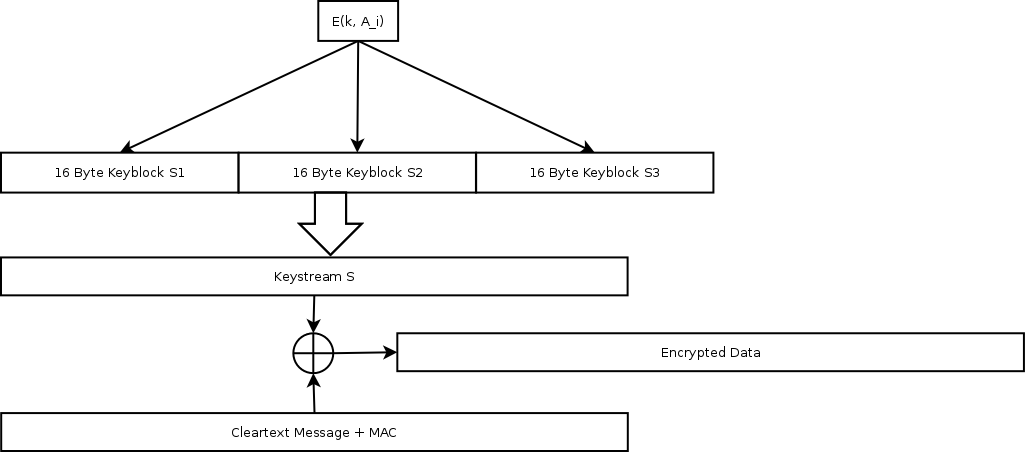
\includegraphics[width=1\textwidth]{figures/CTR.png}
    \caption{CTR Encryption}
    \label{fig:ctr}
\end{figure}

First, keyblocks with 16 byte length each are generated by encrypting the nounce, a flag and a counter with the key. These 
keyblocks are then concatenated and trimmed to the proper length(=length of the message to encrypt). This obtained keystream
is then bitwise xored with the cleartextmessage(which consists of the data and the MAC), yielding the final encryption.


\subsubsection{Decryption and Authenticity Check}

\subsubsection{Attacks on CCM}

FIXME: meet in the middle attack, siehe rfc 3610

\section{Public Key Cryptography}

Public Key Cryptography solves the problem of establishing a secure channel by using an unsecured one.
Here sender and recipients use two different keys: one for encryption, called \textit{public key}, the other
for decryption, called \textit{private key}. This key pair belongs together, hence this scheme is also called \textit{asymmetric} encryption. A key requirement
is that it must be hard
to derive the decryption key from the encryption key. This behavior is achieved by some kind of public known one-way function where it is computationally
easy to calculate the result of $f(x) = y$, but only given $y$, it is computationally - in the domain of processing power and/or memory - hard
to reverse this function to get $x$, although the reverse function may exist in mathematical sense. This is even a desired property. Otherwise
it may facilitate to find the argument that led to the output, i.e. take the constant function, where it is trivial to find the argument.
By that fact, the encryption or public key can be published in some sort of dictionary without compromising the private key. An entity wanting to
send an encrypted message to a receiver can then look up the receiver's public key, encrypt the message and send the resulting
ciphertext to the recipient, who then can decrypt the message. It is remarkable that any algorithm establishing public keys must authenticate it's 
participants, or it will be vulnerable to man-in-the-middle attacks.

\subsection{Discrete Logarithm Systems}

Whitfield Diffie and Martin Hellman were the first who proposed a way to solve the problem for key-exchange by introducing the concept of 
a public-key cryptography when they published their paper \textit{New Directions in Cryptography} back in 1976. The security of this concept
is based on the hardness of the \textit{Discrete Logarithm Problem}. 

With the original Diffie-Hellman algorithm, 2 entities - $A$ and $B$ - use exponentiation over finite fields to agree on a shared secret, which
then can be used parametrize a block or stream cipher. The first step for booth entities is to agree on the set of parameters $\{p, q, g\}$, where $p$ is a 
large prime, $q$ is a prime divisor of $p-1$, and $g$ is a generator of the cyclic group ${Z_p}^*$ in the range $[1, p-1]$. These parameters are not secret and
can thus be sent over an unsecured channel.
Additionally, each entity randomly chooses an integer $x$ from the interval $[1, q-1]$, and calculates the value  $y = g^x \pmod p$. $x$ is the private key,
$y$, which is computationally easy to calculate, is the public key. $A$ sends its public key $y_A \equiv g^{x_A} \pmod p$ to $B$, and $B$ its public key
$y_B \equiv g^{x_B} \pmod p$ to $A$. Due to the characteristics of exponentiation, $A$ and $B$ can now easily derive the shared secret by using it's counterpart's
public key and raising it to the power of it's own private key in the domain of ${Z_p}^*$:

$k_B \equiv {y_A}^{x_B} \equiv {g^{x_A}}^{x_B} \equiv g^{x_A*x_B} \pmod p = k_A \equiv {y_B}^{x_A} \equiv g{^{x_B}}^{x_A} \equiv g^{x_B*x_A} \pmod p $

An eavesdropper that intercepts the initial sent paramter set $\{p, g, q\}$ and the public keys $y_A$ and $y_B$ and that wants to calculate the shared secret
$k_A = K_B$  must therefore the Discrete Logarithm Problem. FIXME: security analysis of DLP

\subsection{Diffie-Hellman based on Elliptic Curves}

\subsection{RSA}

\section{Random Number Generators}

\subsection{Quality / Measurement}

\subsection{Hardware based}

usb stick: 
www.entropykey.co.uk


\section{Attacks on Ciphers}

\subsection{Passive Attacks}

timing attacks - constant time computation

\subsection{Active Attacks}